\chapter{Program Languages, Costs, and Minimality}
\label{ch:languages-costs}

Two programmers replace a six-instruction sequence with four instructions.
The replacement passes every test they run. One programmer says that the new
sequence is shorter. The other says that it is the shortest possible. The
first statement needs a count. The second needs a universe.

That universe is easy to leave implicit. Perhaps an instruction may use any
register, or only registers that are dead at the replacement site. Perhaps a
constant may appear as an immediate, arrive in a register, or be loaded from
memory. Perhaps two instructions with different byte encodings count as the
same operation. On x86-64, a sequence with fewer instructions can occupy more
bytes. On either real machine, a sequence that looks cheap in the ISA manual
can be slow on one processor and fast on another. ``No cheaper program
exists'' has no stable meaning until these choices have been printed beside
the claim.

This chapter constructs that missing universe. We will first make a small
candidate language, then choose a cost, and finally rule out every cheaper
program in it. The worked case is deliberately small enough to check with a
pencil. Its value is not the difficulty of adding two. Its value is that no
premise can hide in the machinery.

\begin{keyidea}[title={A minimality claim has three named parts}]
A program is minimal only relative to a candidate language, an equivalence
contract, and a cost order. Change any one of the three and the claim changes.
The ISA name by itself supplies none of them.
\end{keyidea}

\section{From clever sequences to complete searches}

Programmers have always looked for shorter or faster ways to express a fixed
calculation. A compiler performs the same work mechanically when it replaces
an expensive instruction pattern with a cheaper one. The old name
\term{peephole optimization} describes the scale: look through a small window
at a few adjacent instructions, recognize a pattern, and substitute another.
The window is small, but the question inside it is already mathematical. Do
the old and new programs agree for every allowed input?

In 1987 Henry Massalin described a \keyterm{superoptimizer}: a system that
searches for the smallest program implementing a function rather than relying
only on a catalog of known rewrites.\autocite{massalin1987} Later work made
peephole superoptimization more systematic and made complete searches scale
through better decomposition and parallelism.\autocite{bansalaiken2006,lubodik2025}
These systems differ in language, search method, and cost. They share a
pressure that matters here: the word \emph{smallest} forces the search space
into the statement.

A search can serve at least three different goals.

\begin{enumerate}
\item It can find any program that meets a specification.
\item It can improve on a known program under a chosen cost.
\item It can show that no cheaper candidate meets the specification.
\end{enumerate}

The first two goals need a witness. The third needs coverage. If a search
finds a three-instruction program, then a three-instruction program exists.
It does not follow that two instructions are impossible. To establish that
lower bound, every candidate of cost zero, one, and two must be represented
and rejected, or a separate argument must rule out the same space.

That asymmetry explains why optimization practice often stops after finding a
good sequence. A witness is compact and cheap to replay. A failed search may
mean that the tool timed out, its grammar omitted the needed operation, its
encoding was wrong, or there truly is no candidate. Only the last reading is
a lower bound, and it is the reading that requires the most care.

\section{Print the language before searching it}

A \keyterm{candidate language} is the exact set of programs allowed to compete
with the reference program. For a bounded search, we want this set to be
finite and mechanically enumerable. An ISA manual is an input to its design,
not the language itself. The manual may describe privileged instructions,
optional extensions, hundreds of operand forms, implementation-dependent
features, and behaviors outside the replacement site. A theorem about a
selected scalar fragment must say selected scalar fragment.

The most useful language declaration answers eight questions.

\begin{definition}[title={Candidate-language contract}]
A bounded candidate-language contract declares:
\begin{enumerate}
\item the decoded instruction forms that may occur;
\item the operand forms and widths for each instruction;
\item the registers, constants, and temporary storage available at entry;
\item the memory regions candidates may read or write;
\item the legal starting addresses and decoding policy;
\item the precondition on initial states;
\item the maximum program length or cost bound; and
\item the observation used to compare final behavior.
\end{enumerate}
Together these clauses determine which byte strings or decoded sequences are
candidates and what it means for one to work.
\end{definition}

The order matters less than the completeness. A register restriction without
an operand restriction may still admit an implicit accumulator. A ban on
stores does not ban loads. A list of decoded operations does not say whether
all their encodings are admitted. A maximum of four instructions does not
bound four x86-64 instructions to one fixed byte length. Each clause closes a
different door.

\begin{figure}[htbp]
\centering
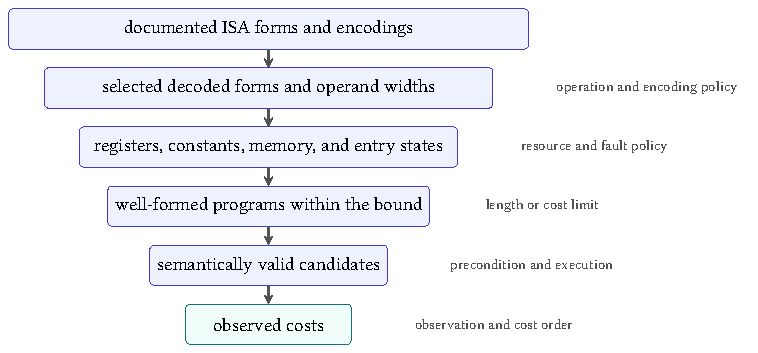
\includegraphics[width=0.96\textwidth]{figures/candidate-language-funnel}
\caption{A bounded search does not range over an ISA name. Each declared
choice narrows the source universe until a finite set of observed candidate
behaviors remains.}
\figalt{A funnel narrows ISA forms through operands, resources, bounds, semantics, observation, and cost.}
\label{fig:candidate-language-funnel}
\end{figure}

\subsection{Decoded forms and byte encodings}

There are two sound ways to start. An \term{extensional} language prints every
allowed decoded instruction instance. This is pleasant for a dozen
candidates and impossible for a million. An \term{intensional} language gives
a finite grammar: choose an operation from this list, a destination from this
set, and each source from its permitted set. The grammar must expand to the
same concrete instances the encoder or symbolic translator uses.

Decoded instructions and byte strings are not interchangeable. A0 assigns
one four-byte encoding to each legal decoded instance, so the bridge is
simple. RV64I uses fixed 32-bit base instructions, but the compressed
extension adds 16-bit encodings and its own operand restrictions. x86-64 may
encode closely related operations with different prefixes, immediate widths,
or addressing forms. A search over meanings can quotient duplicate encodings
when cost ignores bytes. A byte-minimal search cannot.

Canonicalization can reduce work without weakening a claim, but only when the
discarded candidates are genuinely redundant. Suppose addition is
commutative and both sources are pure registers. Keeping only
\code{add r0,r0,r1} and dropping \code{add r0,r1,r0} preserves the possible
result functions. If the two forms have different encodings, fault behavior,
or costs, that quotient is no longer harmless. The proof obligation for a
search-space reduction is the same as for any other rewrite: every removed
candidate must have a retained representative with the same observed
behavior and no greater cost.

\subsection{Constants are resources}

The expression \(x+1\) looks as though it contains a free constant. Machines
do not receive constants from typography. A one may be encoded in an
immediate field, held in an entry register, constructed from zero, read from a
literal pool, or obtained through a special instruction. Those routes consume
different instructions, bytes, registers, and memory permissions.

Consider a language with only register-register addition. If \(r_1=1\) is an
entry premise, then \code{add r0,r0,r1} computes \(x+1\) in one instruction.
Remove that premise and the same text reads an arbitrary second input. Add an
immediate form and the register is unnecessary. The function has not changed;
the candidate language has.

\begin{warning}[title={Do not smuggle a constant through the harness}]
A test harness that initializes a register or memory cell has granted every
candidate access to a resource. State that resource in the precondition and
language contract. Otherwise the search and the printed claim concern
different machines.
\end{warning}

Temporaries work the same way. A dead register at a compiler replacement site
may be available as scratch. A live register may be used only if the candidate
restores it and the observation checks that restoration. Stack space, flags,
and vector registers are not free merely because a calling convention makes
some of them caller-saved. The local context decides which changes are
observable.

\subsection{Memory policy is more than yes or no}

A candidate that may use memory needs a region, permissions, alignment rule,
aliasing policy, and fault policy. ``One temporary stack slot'' should name
its address relation to the stack pointer, its width, and whether it can
overlap any input or output. If a reference program never faults but a
candidate can fault on an allowed state, normal-result agreement does not
rescue the candidate.

Memory also threatens finiteness. If an address immediate may be any word,
the grammar has \(2^w\) choices at width \(w\). That is finite in mathematics
and useless as a naive enumeration. A language may restrict addresses to a
declared set of symbolic regions, or it may encode address choices in a
solver. Either choice belongs in the scope. ``Memory instructions permitted''
is not enough information to reproduce the set.

\section{The equivalence contract inside the search}

Chapter~\ref{ch:equivalence-refinement} defined program agreement relative to
a precondition and an observation. A minimality search inherits that entire
contract. Let (S) be the specification program or function, (P) a
candidate, (A(s)) the allowed-input predicate, and (O) the observation.
The candidate works when
\[
  \forall s,\quad A(s)\Longrightarrow O(P(s))=O(S(s)).
\]
If execution can trap, halt, or diverge, (O) must retain whichever behavior
classes the replacement context can detect. A result-only projection may be
appropriate for a pure straight-line exercise. It is too weak for a compiler
rewrite when the continuation can read flags or observe a fault.

This universal condition is where testing stops. Tests sample states. The
candidate must work on every state allowed by (A). For a tiny width, direct
enumeration can check all inputs. At width 64, symbolic bit-vector reasoning
can represent all \(2^{64}\) inputs without listing them one by one. The
symbolic formula is still accountable to the instruction semantics and the
observation that produced it.

The language and equivalence contract interact. If candidates may use a
temporary register, then the observation must say whether its final value
matters. If candidates may access memory, the precondition must supply valid
memory and the observation must compare the permitted effects. If a candidate
may be shorter than the reference, the harness must define where execution
stops rather than letting it run into whatever bytes happen to follow.

\begin{example}[title={One omitted flag changes the winner}]
Suppose an A0 sequence clears \(r_0\) with arithmetic and leaves \(Z=1\), while
a shorter move also writes zero but leaves different condition bits. Under an
observation containing only \(r_0\), the move may win. Under an observation
that also contains (Z,N,C,V), it does not. Neither answer corrects the
other. They answer different replacement questions.
\end{example}

\section{Cost is a function, not an adjective}

A \keyterm{cost model} maps a candidate program and its declared context to an
ordered value. The simplest model counts instructions:
\[
  C_{\mathrm{inst}}(P)=|P|.
\]
For A0's fixed-width encoding, byte length is four times instruction count,
so the two costs induce the same order. This convenience is a feature of the
teaching machine, not a universal property of instruction sets.

For a variable-length encoding, define
\[
  C_{\mathrm{bytes}}(P)=\sum_{i=1}^{|P|} b(P_i),
\]
where \(b(P_i)\) is the encoded length of instruction \(P_i\).
A two-instruction x86-64 sequence may occupy fewer bytes than one instruction
with a long immediate and addressing fields. An RV64 search that admits the
compressed extension can similarly prefer two 16-bit instructions over one
32-bit instruction only if the cost order permits a tie or includes another
component; it cannot pretend that instruction count and byte count are the
same measurement.

An abstract weighted model assigns a declared weight to each instruction
instance or class:
\[
  C_{\mathrm{weight}}(P)=\sum_i W(P_i).
\]
Weights can represent an engineering preference, but their interpretation
must be named. A multiply might receive weight four and an add weight one.
That does not say the multiply takes four cycles on a real processor. It says
the theorem uses the printed table.

\begin{table}[htbp]
\centering
\caption{Three cost models can order the same candidates differently. The
numbers are illustrative, not measurements of a processor.}
\begin{tabular}{lccc}
\toprule
Candidate & Instructions & Bytes & Declared weight \\
\midrule
\(P_A\): one rich instruction & 1 & 7 & 4 \\
\(P_B\): two compact instructions & 2 & 4 & 2 \\
\(P_C\): three simple instructions & 3 & 6 & 3 \\
\bottomrule
\end{tabular}
\label{tab:cost-orders}
\end{table}

The table has three different winners: \(P_A\) by instruction count, \(P_B\)
by bytes and declared weight, and no universal winner independent of the
question. Calling one sequence ``better'' would discard exactly the
information a minimality statement needs.

Cost can also depend on the replacement site. A sequence that needs one dead
temporary may be admissible where that register is free and inadmissible where
it carries a live value. Saving and restoring the register changes both the
candidate and its cost. Alignment can change encoded padding or the placement
of an x86-64 instruction across a fetch boundary. A literal already present in
nearby memory is a different resource from a literal that the replacement
must introduce. For this reason, the most general cost has the shape
\(C(P,K)\), where \(K\) records the declared context. A context-independent
model is still useful; it simply fixes or ignores those terms and says so.

\subsection{Latency and throughput need a processor}

The ISA defines architectural behavior. It does not fully define how many
cycles a concrete processor spends on a sequence. Latency can depend on
operand values, cache state, branch prediction, instruction alignment,
microarchitectural generation, and the instructions around the replacement.
Throughput asks a different question from dependency-chain latency. A model
for either must name the processor data, scheduling assumptions, and context
used to combine individual costs.

Measured performance introduces noise and environmental state. A benchmark
can compare two sequences on a named machine under a named protocol. It
cannot by itself establish a universal minimum over all programs, and a
minimum in an abstract schedule model need not be the fastest sequence on
silicon. The honest result is often a pair: a theorem about the model and a
measurement about the machine.

\subsection{Orders, ties, and several objectives}

Costs need not be single numbers. The adjective \keyterm{lexicographic} means
that we compare the first component and consult the next one only to break a
tie. A cost with this order might minimize bytes first and then instructions
among equal-byte candidates:
\[
 C(P)=\bigl(C_{\mathrm{bytes}}(P),C_{\mathrm{inst}}(P)\bigr).
\]
Lexicographic order makes the first component decisive. A Pareto order instead
keeps every candidate for which no other candidate is at least as good in all
components and strictly better in one. The result is a frontier, not one
winner.

Ties matter. Two different programs can have the same minimum cost. A search
for \emph{a} minimum witness may return either. A search claiming uniqueness
must rule out every other equivalent candidate at the same cost after stating
which syntactic differences count. Register renaming, commutative operands,
and duplicate encodings can make uniqueness a much stronger claim than
minimality.

\begin{goingdeeper}[title={Well-founded cost orders}]
A lower-bound search works by exhausting costs below a witness. This argument
needs a cost order with no infinite descent in the searched region. Natural
numbers and finite lexicographic tuples of natural numbers have that property.
Arbitrary real-valued estimates or partially ordered profiles need a more
careful statement of what ``all cheaper candidates'' means.
\end{goingdeeper}

\section{An upper bound and a lower bound must meet}

Let (L) be the candidate language, (E(P,S)) the equivalence condition, and
\(C(P)\) the cost. A witness \(P^*\in L\) with \(E(P^*,S)\) supplies an upper
bound \(C(P^*)\). Minimality also needs
\[
  \neg\exists P\in L,\quad C(P)<C(P^*)\ \land\ E(P,S).
\]
That second formula is the lower bound. It says that the cheaper region is
empty of working programs. The two statements do different jobs and deserve
different checks.

\begin{figure}[htbp]
\centering
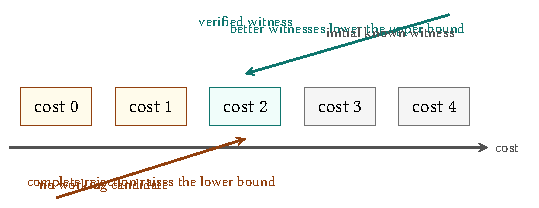
\includegraphics[width=0.92\textwidth]{figures/upper-lower-meet}
\caption{A witness lowers the best known upper bound. Exhausting or refuting
cheaper cost strata raises the lower bound. Minimality follows only when the
two meet under one language and equivalence contract.}
\figalt{A cost axis shows rejected cheaper layers rising to meet a verified witness upper bound.}
\label{fig:upper-lower-meet}
\end{figure}

A common search alternates the two sides. It begins with a reference program
as an upper bound, searches lower costs, and replaces the witness whenever it
finds an improvement. When every smaller stratum has been rejected, the last
witness is minimal. Another search asks for cost zero, then one, then two, and
stops at the first satisfiable cost. That method is complete only if each
earlier query covered its entire cost stratum.

Timeouts do not raise a lower bound. Nor does a solver's failure to find a
candidate unless the algorithm's completeness and termination for that query
have been established. ``No result in one hour'' is a measurement of the
search, not a property of the language.

\section{A tiny A0 lower bound}

We now make every choice explicit. Fix an A0 word width \(w\geq2\). At entry,
\(r_0=x\) is the input and output register, and \(r_1=1\) is a read-only
resource. Other registers and memory are unavailable. Candidates are
straight-line sequences over these six decoded instances:

\begin{codelisting}[language={},caption={The complete tiny candidate alphabet}]
mov r0, r0          mov r0, r1
add r0, r0, r0      add r0, r0, r1
add r0, r1, r0      add r0, r1, r1
\end{codelisting}

Every instruction executes normally in a valid code region. The harness stops
after the declared number of instructions. The observation contains only the
final value of \(r_0\) and normal completion; it ignores \(pc\) and the A0
condition bits. Cost is instruction count. The specification is
\[
  S(x)=x+2\pmod {2^w}.
\]
The task is to find the least cost among candidates of length at most two.

There is a two-instruction witness:

\begin{codelisting}[language={},caption={A two-instruction witness for adding two}]
add r0, r0, r1
add r0, r0, r1
\end{codelisting}

After the first step, \(r_0=x+1\). The instruction does not change \(r_1\), so
the second step produces \(x+2\), with all arithmetic taken modulo \(2^w\).
This replay establishes the upper bound two.

The lower bound is small enough to see as a table. A zero-instruction program
returns (x). The six one-instruction instances return only the following
five functions; the two mixed-source additions coincide because word
addition is commutative.

\begin{table}[htbp]
\centering
\caption{Every program below cost two in the tiny A0 language. A single input
separates each observed function from \(x+2\).}
\begin{tabular}{lll}
\toprule
Candidate form & Final \(r_0\) & Separating input \\
\midrule
empty or \code{mov r0,r0} & (x) & any (x) \\
\code{mov r0,r1} & \(1\) & \(x=0\) \\
\code{add r0,r0,r0} & \(2x\) & \(x=0\) \\
\code{add r0,r0,r1} or reversed & \(x+1\) & any \(x\) \\
\code{add r0,r1,r1} & \(2\) & \(x=1\) \\
\bottomrule
\end{tabular}
\label{tab:a0-add-two-lower-bound}
\end{table}

\begin{proofkit}[title={Reader proof: no cheaper candidate adds two}]
At cost zero the output is \(x\), which differs from \(x+2\) because
\(2\not\equiv0\pmod {2^w}\) when \(w\geq2\). At cost one, the table is a
complete split over the six allowed instruction instances. The constant one
differs from the specification at \(x=0\). The function \(2x\) also differs
there. The function \(x+1\) differs for every input because one and two are
distinct words. The constant two differs at \(x=1\). Thus no candidate of
cost less than two works for every input. The two-step witness works for every
input, so the minimum instruction count in this printed language is two.
\end{proofkit}

\begin{figure}[htbp]
\centering
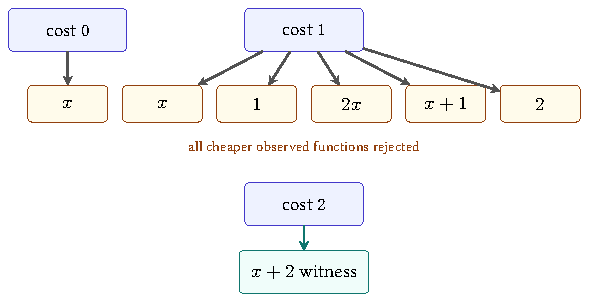
\includegraphics[width=0.94\textwidth]{figures/a0-xplus2-search}
\caption{The lower-bound argument classifies every observed function below
cost two. The witness occupies the first cost stratum that contains the
specification.}
\figalt{Cost zero and one lead to five rejected functions; cost two contains the x plus two witness.}
\label{fig:a0-xplus2-search}
\end{figure}

The case now has a complete reader argument for its teaching language. It is not yet a
machine-backed book result: no current object binds this exact grammar,
enumeration, checker, and negative control. That distinction matters even
when the mathematics fits on half a page. The later evidence route must check
the bytes and semantics it claims, not borrow confidence from this table.

\subsection{Why every clause mattered}

The width premise excludes \(w=1\), where \(2\equiv0\pmod2\) and the empty
program already implements \(x+2\). Making \(r_1\) read-only prevents the
first instruction from destroying the constant used by the second. Ignoring
condition bits permits the two-step witness to satisfy a result-only
specification; a stronger observation would have to specify the desired final
conditions. Banning immediates excludes a one-step \code{addi} form. Banning
memory excludes a table lookup or loaded constant. Limiting the register set
keeps the one-step alphabet exactly as printed.

Add just one instruction, \code{addi r0,r0,2}, and the old lower bound no
longer describes the new language. This is not a counterexample to the
argument. It is a reminder that minimality does not float above scope.

\begin{tryit}[title={Break the claim cleanly}]
Extend the alphabet with \code{movi r0,2}. Does the minimum change? Now extend
it with \code{addi r0,r0,2}. Explain why the first extension leaves the lower
bound intact while the second supplies a cheaper witness. State the modified
language before giving either answer.
\end{tryit}

\section{Turning enumeration into evidence}

The pencil proof used a useful compression: six one-step programs produced
only five observed functions. A program search can exploit the same idea.
Breadth-first enumeration begins at the empty program, extends each retained
prefix by every instruction instance, executes or symbolizes the result, and
groups candidates with equal observed behavior. For a deterministic finite
machine at a tiny width, a complete truth table can serve as the behavior key.

Suppose two prefixes have the same observed state transformer and the same
available resources, while one costs no more than the other. Any common
suffix gives the same observed result, so the more expensive prefix can be
discarded. This is semantic quotienting. It can shrink a search dramatically,
but the equality used for grouping must retain every state component that a
future suffix can read. Grouping only by current \(r_0\) would be unsound if a
later instruction can read flags, \(r_1\), or memory.

For larger widths, a solver can represent instruction choices and symbolic
states. A bounded query asks whether there exist decoded instructions and an
allowed input relation such that the candidate meets the universal
specification. The quantifier structure needs care. To refute equivalence of
a fixed candidate, a solver searches for an input where the outputs differ.
To synthesize a candidate that works for all inputs, the conceptual form is
\(\exists P\,\forall s\). Many practical systems alternate candidate
generation with counterexample discovery rather than handing that formula to
one solver unchanged.

\subsection{Counterexample-guided search}

A counterexample-guided loop keeps a finite set of test inputs. It finds a
candidate that works on those inputs, then asks a \keyterm{verifier}, the
checker for universal agreement, for an allowed input where the candidate
fails. A counterexample joins the test set, and the loop repeats. If the
verifier finds none under a sound complete route, the
candidate meets the universal contract. If no candidate can satisfy the
accumulated examples, the current cost stratum may be empty, but the lower
bound still depends on how candidate choices and universal correctness were
encoded.

This loop turns failures into useful information. The values \(x=0\) and
\(x=1\) in Table~\ref{tab:a0-add-two-lower-bound} are exactly such separating
inputs. They eliminate whole classes of candidate functions. The search is
not merely trying programs; it is learning which distinctions the
specification requires.

\subsection{What a checkable lower bound must retain}

A durable result needs more than a final line saying that a solver returned an
unsatisfiable verdict. The evidence package should retain enough information to reconstruct
the claim:

\begin{enumerate}
\item a serialized candidate-language contract;
\item the specification, precondition, observation, and cost order;
\item the exact decoder and semantic version or digest;
\item the formula for every cheaper cost stratum, or a reproducible generator;
\item a witness at the claimed minimum cost;
\item a checkable refutation for each cheaper satisfiability query when the
solver route can export one; and
\item a negative control that corrupts a witness, formula, or proof and is
rejected.
\end{enumerate}

The witness checker and lower-bound checker should fail for different reasons.
Change the second add in the A0 witness to \code{add r0,r0,r0}; replay should
find an input where the result differs. Add a legal one-step \code{addi}
candidate without regenerating the cheaper-space formula; a language-closure
check should catch the mismatch before a solver result is trusted. Truncate a
refutation; the proof checker should reject it. These attacks test three
different links.

\begin{warning}[title={A solver verdict is not a portable lower bound}]
An unsatisfiable verdict reports what one solver said about one formula. A checked
refutation can support that formula's unsatisfiability. Neither establishes
that the formula represents the printed candidate language unless the
encoding bridge is also checked.
\end{warning}

\section{Negative controls for search claims}

The most revealing negative control gives the checker something it ought to
accept but the claimed lower bound says cannot exist. Add a known cheaper
witness to the language, rebuild the search space, and require the
lower-bound check to fail. This tests candidate coverage and not merely proof
parsing.

Other controls target nearby faults:

\begin{itemize}
\item omit one operand form from enumeration while leaving it in the printed
grammar;
\item reverse one subtraction operand in the symbolic semantics;
\item observe \(r_0\) but accidentally drop a required flag;
\item allow a temporary in synthesis but freeze it in verification;
\item compute byte cost from decoded mnemonics instead of actual encodings;
\item accept a solver log after deleting the load-bearing proof bytes; or
\item change the precondition between the witness and lower-bound queries.
\end{itemize}

A positive run says the components agree on the intended instance. A
negative control shows that at least one nearby wrong instance crosses a
failure boundary. It does not prove the checker has no other bugs. It makes
the checking claim falsifiable and gives future maintainers a precise alarm.

\section{From A0 to RV64 and x86-64}

A0 makes instruction-count minimality unusually clean. Its instructions have
one width, its first scalar model has a small explicit state, and the book
owns its definition. The real-ISA slices add obligations before they add
glory.

For an RV64I scalar search, name the base ISA version, permitted extensions,
architectural integer width, privilege assumptions, and exact operand forms.
Decide whether compressed
instructions compete. State how illegal encodings, misaligned control flow,
loads, stores, and traps enter the observation. If the language includes only
register-register integer operations, say so. ``RISC-V program'' is much too
large a noun.

For x86-64, decode mode and encoding are central. Name 64-bit mode, selected
instruction forms, operand and address sizes, allowed prefixes, register
classes, memory forms, and the portions of the flags register that matter. Decide how
partial-register writes and implicit operands enter the state. If cost is
bytes, retain the actual encoding. If cost is instruction count, explain how
multiple encodings of one decoded instruction are handled.

Neither slice authorizes a claim about RISC against CISC. One may expose an
interesting contrast: a regular fixed-width language makes byte cost easy to
relate to instruction count, while a variable-length language makes encoding
part of the optimization problem. That is a statement about declared
features, not two architectural essences.

Prior systems have claimed instruction-sequence optimality under their own
languages and models.\autocite{bansalaiken2006} The contribution sought here
is therefore not a priority slogan. It is a per-instance route in which the
reader can inspect the language, replay the witness, check the cheaper-space
refutations, and break the checker with a negative control.

\section{The Axeyum route, in the right order}

The live Axeyum checkout already supplies useful lower layers: fixed-width
bit-vector terms, solver connections, propositional encodings, proof checking
components, and kernel-facing evidence machinery. It does not yet supply a
reusable A0 decoder and transition system, nor complete RV64 or x86-64
packages. We should not place a Python convenience function over that gap and
call the result an ISA proof.

The first implementation route should follow the dependency order already
visible in the reader argument.

\begin{enumerate}
\item Define the candidate-language data types in Rust: decoded forms,
resources, precondition, observation, bound, and cost.
\item Connect those forms to an executable A0 decoder and step semantics.
\item Enumerate the tiny language and replay each candidate concretely at a
small width, including the zero- and one-instruction layers above.
\item Translate the same semantics to Axeyum bit-vector expressions and check
candidate equivalence by searching for a counterexample input.
\item Emit a canonical record of the language, witness, formula digests, and
cheaper-stratum results.
\item Add proof-export and independent checking where the selected solver
route supports it, then add mutations that must fail.
\item Expose a small Python interface only after Rust owns these meanings and
the evidence record.
\end{enumerate}

Python is useful for teaching and orchestration. A reader should be able to
construct the six-form language, request a bounded search, inspect the
witness, and print a counterexample without writing Rust. The Python object
must serialize to the same canonical contract the Rust checker reads. It
must not reimplement instruction semantics or decide what a successful proof
means.

The teaching display should expose the search strata as well as the winner.
For each cost below the upper bound, it can show the number of syntactic
candidates, the number rejected by typing or resource rules, the number
eliminated by concrete counterexamples, and the obligations sent to the
solver. Those counts make the lower-bound argument visible. They also catch a
damaged enumerator: a suspiciously empty stratum is a question, not a gift.

One small witness from every rejection class is useful. A malformed operand
explains the grammar. A clobbered scratch register explains the observation.
A boundary input explains semantic failure. The retained examples teach why
the candidate language and harness are part of the theorem rather than setup
around it.

\begin{codelisting}[language=python,caption={The intended shape of a future teaching interface}]
# Illustrative API: this interface is not yet implemented.
language = CandidateLanguage.a0(
    width=4,
    forms=["mov.rr", "add.rrr"],
    registers=["r0", "r1"],
    constants={"r1": 1},
    writes=["r0"],
    observation=["normal", "r0"],
    max_instructions=2,
)
result = search_minimal(language, spec="r0_out == r0_in + 2")
result.replay_witness()
result.check_lower_bound()
\end{codelisting}

The comment is part of the lesson: the interface is a design target, not a
reported capability. Once it exists, the book should replace illustrative
code with an executable example and bind any machine-backed result to the
exact Axeyum revision and checker route.

The real-ISA layers come later. First establish that decoded bytes and A0
steps agree, then lift selected RV64 forms, then selected x86-64 forms. Only
after those semantic bridges survive their own negative controls should the
same minimality engine range over them. The search engine is not the hard
foundation. Meaning is.

\section{Where the model stops}

No claim here ranges over all programs on any architecture. The model excludes
self-modifying code, concurrency, interrupts, privileged state, caches,
speculative execution, and whole-program link layout. It does not infer
hardware speed from an instruction count or turn a timeout into a lower bound.

Even within straight-line scalar code, a model may omit a useful instruction,
constant route, temporary, or encoding. Such an omission does not make the
bounded result false. It makes the result narrower. The remedy is to publish
the language so another person can extend it and see whether the minimum
changes.

The construction has a modest and surprising reach. Its language is finite
because we chose the pieces and the bound. Once those choices are
fixed, checking every cheaper program can support a statement about all of
them. A small list of instructions becomes a universal negative, but only
inside the border we drew.
Publishing that border lets the next search enlarge it without misquoting the
result already obtained.

\section{Exercises}

\begin{enumerate}
\item \textbf{Execute.} At width four, replay the two-instruction A0 witness
for inputs \(0,1,7,14,\) and \(15\). Record the intermediate and final \(r_0\).

\item Enumerate all six one-instruction candidates in the tiny language
without quotienting commutative additions. Confirm that their observed
functions match Table~\ref{tab:a0-add-two-lower-bound}.

\item \textbf{Prove.} Generalize the reader argument from adding two to adding
(k) by repeated addition of the entry constant one. State a language in
which (k) instructions are minimal, or explain why the present language
admits a shorter construction for some (k).

\item Find every place the width premise \(w\geq2\) enters the lower-bound
argument. Give the exact result at width one.

\item \textbf{Break.} Add \code{addi r0,r0,2} to the language. Write the new
one-step function table and identify the failed sentence in the old proof.

\item Add \code{sub r0,r0,r1}. Does it create a cheaper witness for \(x+2\)?
Does it create new observed functions? Answer for width two and width three.

\item Change the observation so that it includes A0's (Z,N,C,V). Define the
specification's desired final conditions, then determine whether the old
witness still works.

\item Allow \(r_1\) to be overwritten and add \code{mov r1,r0} plus addition
forms writing \(r_1\). State the preservation rule needed if the caller
observes \(r_1\) at exit.

\item Give two concrete x86-64 instruction sequences that would be ordered
differently by instruction count and encoded byte length. Pin the mode and
write the bytes before comparing them.

\item For RV64, compare a language containing only 32-bit RV64I instructions
with one that admits a named compressed extension. Which parts of the
candidate-language contract must change?

\item Design a lexicographic cost that minimizes memory accesses, then bytes,
then instruction count. Give two candidates tied on the first component and
separated by the second.

\item Construct three abstract candidates whose costs form a Pareto frontier
under bytes and latency. Explain why the frontier has no single minimum
without another policy choice.

\item \textbf{Act as the checker.} Mutate the second instruction of the A0
witness in three ways. For each mutation, give the smallest separating input
you can find and the observed wrong result.

\item Design a negative control that detects omission of one legal operand
form from an enumerator. State which component must fail before the solver is
called.

\item A search reports no candidate of cost at most three after a one-hour
timeout. List the additional evidence needed before this observation can
support a lower bound.

\item State the semantic condition under which two search prefixes may be
grouped by their current state transformer. Give a counterexample to grouping
only by \(r_0\) when later instructions can read \(Z\).

\item \textbf{Transfer.} Write the candidate-language contract for replacing
a two-instruction RV64I integer sequence at one compiler site. Include live
registers, extensions, memory, traps, observation, and cost.

\item Design the first Axeyum evidence record for the tiny A0 search. Include
canonical language bytes, semantic revision, witness, formula digests,
checker result, and one negative-control mutation. Mark which fields the
Python layer may display and which meanings Rust must own.
\end{enumerate}
